\section{Experiments}
\label{sec:experiments}
This section includes the detailed description of our experiments conducted to analyze the impact of database cracking on query execution performance. We use a similar setup for all performance evaluations. Our main focus is to study the impact of cracking the SELECT operator in memory. In order to identify relative performance, we ran the same set of queries on the same column for all cracker index implementations and compared the results to two baselines: (1) simple scanning time when all column values are scanned and filtered linearly and (2) sorted-column scanning when the column is sorted upfront upon the arrival of the first query and searched for range values using binary search. Overall, we found that in our experimental environment for large workloads (10,000 - 20,000 queries), all three cracker implementations take less time to perform range scans than the baseline.

\subsection{Experiment setup}

\textbf{Hardware:} We used the Amazon AWS server (8 GB memory) and MIT Athena computers (40 GB memory). \\
\textbf{Dataset:} All experiments were conducted on a column with one million distinct tuples of range 1 to 10${^6}$. \\
\textbf{Workload:} We measured the performance of 10,000 and 20,000 randomly generated queries with varying selectivity.\\
\textbf{Query ranges:} We used open (single predicate), closed (lower and upper predicates) and mixed (randomly chosen to be either open or closed) query ranges.\\
The predicate values are chosen randomly from the range 1 to 10${^6}$.
\textbf{Selectivity:} Our query selectivity values are 0.01 and 0.001. \\
\textbf{Minimum Partition Size: } We enforced the minimum partition size to be 100 and 1000 tuples. The cracker index could potentially become very large for non-repetitive queries, and dividing columns further into small pieces would become highly costly. Therefore, we experimented with minimum partition sizes in order to restrict further column cracking.

\subsection{Performance of cracking index implementations}
We started our experiments by running 10,000 and 20,000 queries with varying ranges, such as single, mixed, and double ranges, without particular choice of the selectivity or minimum partition size. Figures \ref{fig:single10000} and \ref{fig:double10000} show the cumulative response time for each of our cracker index implementations, as well as baseline performances of simple scanning and sorted-column scanning for the workload of size 10,000. We observe that any cracking index implementation outperforms the simple scanning by at least two-fold. The initially high cracking cost is immediately balanced out as the number of queries grow, suggesting that cracking allows faster query execution in the long run. Moreover, note that single (open-ended) ranges require a column to be partitioned once, while double ranges require a column to be partitioned twice. Therefore, we assume that the linear predecessor/successor search time starts impacting the performance of Hash Map, which is no longer the best performing cracker index implementation. Additionally, despite the fact that AVL Tree has logarithmic cost for all operations, it is not outperforming the other two implementations, agreeing with our hypothesis about the costly tree rebalancing operations.

\begin{figure}[h]
\centering
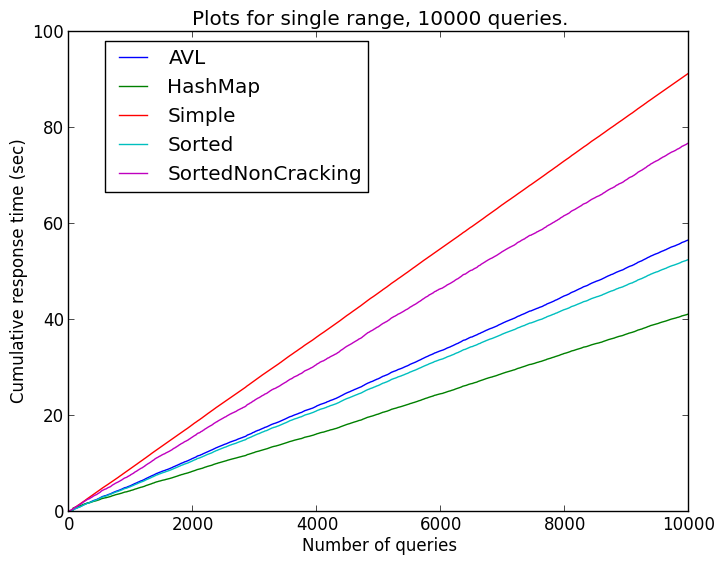
\includegraphics[width=8cm]{figures/single10000}
\caption{Measurement of the cumulative query execution time for three Cracker Index implementations, labeled as AVL, HashMap, and Sorted, as well as simple scanning, labeled as Simple, and sorted-column scanning, labeled as SortedNonCracking. The ranges include only $\textless$, $\leq$, $\textgreater$, $\geq$. The workload size is 10,000 queries, selectivity is 0.01, the minimum partition size is not enforced.}
\label{fig:single10000}
\end{figure}

\begin{figure}[h]
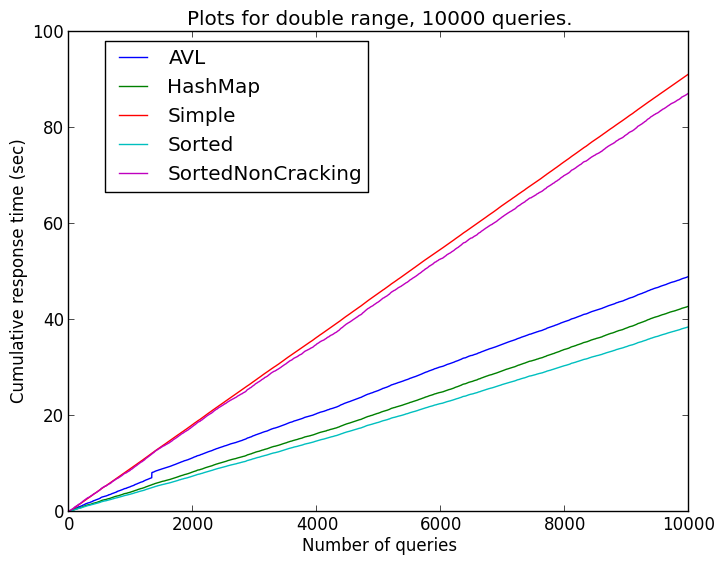
\includegraphics[width=8cm]{figures/double10000}
\caption{Measurement of the cumulative query execution time for three Cracker Index implementations, labeled as AVL, HashMap, and Sorted, as well as simple scanning, labeled as Simple, and sorted-column scanning, labeled as SortedNonCracking. The ranges include only $\textless\textless$, $\leq\textless$, $\textless\leq$, $\leq\leq$. The workload size is 10,000 queries, selectivity is 0.01, the minimum partition size is not enforced.}
\label{fig:double10000}
\end{figure}

\subsection{Varying minimum partition size and selectivity}
In \cite{idreos_2007} authors mentioned that restricting minimum partition size of the column  should be a disk page size or cache line. Since our database implementation is simplified and does not have a notion of page or cache, we enforced the minimum partition size to be a certain fraction of the column size. Particularly, we set it to be either 10 tuples, 100 tuples and unrestricted number of tuples. We found that varying minimum partition size does not have a significant impact on the performance for any of three cracker index implementations. However, we believe that experiments conducted on a more complex and fully developed database could offer more insightful results. \\
We have reached to the conclusion that varying selectivity does not affect the query execution time. Particularly, we assume that lower selectivity ranges will require the same amount of cracking as a higher selectivity ranges, nevertheless, the data access time will dominate in the overall performance. However, since in our simplified database all operations are in-memory operations, we do not account for any disk reads and seeks. Our findings partially agree with results achieved in \cite{schuhknecht_2014}, but in order to fully corroborate this hypothesis, more experiments need to be performed. Our experimental setup limited the scope of experiments required to further investigate the connection between the selectivity and cracking performance.


